\documentclass[11pt]{article}
\usepackage[left=2cm,right=2cm,top=2cm,bottom=2cm]{geometry} 
\geometry{letterpaper}
\usepackage{amssymb}
\usepackage{amsmath}
\usepackage{xcolor}
\usepackage{hyperref}

% = Customize Section Headings =
\usepackage[noindentafter]{titlesec}    % default to noindent after
% sections
\usepackage{graphicx}
\usepackage{hyperref}
\titleformat{\textbf}[runin]{\bf}{\small}{\compact}{}[]
\titleformat{\section}{\bf}{\large}{\compact}{}[]
\titlespacing{\section}{0pt}{20pt}{2pt}
\titlespacing{\textbf}{1pt}{8pt}{5pt}

% = Common Astrophysics Symbols =
\newcommand{\rsol}{R_\odot}
\newcommand{\msol}{M_\odot}
\newcommand{\lsol}{L_\odot}
\newcommand{\E}[1]{\hspace{-0.01in}\times\hspace{-0.02in}10^{#1}}  % Scientific notation, '3\E{8}' --> '3x10^8'
\newcommand{\sol}[1]{{\noindent\color{blue} #1}}     % Solutions in blue
\newcommand{\power}[2]{\ensuremath{#1\times 10^{#2}}}

\newcommand{\note}[1]{{\noindent\color{red} \textbf{#1}}} % Notes in red
\newcommand{\trf}[1]{\textrm{\footnotesize{#1}}}
\newcommand{\trt}[1]{\textrm{\tiny{#1}}}
\newcommand{\then}{ \hspace{0.1in} \Longrightarrow \hspace{0.1in} }

\newcommand\plotoneman[2]{\centering \leavevmode
  \includegraphics[scale=#2]{#1}}

  %\includegraphics[width=#2\linewidth]{#1}}

\renewcommand{\section}[1]{\textbf{\underline{#1}}}

% = Setup Header =
\usepackage{fancyhdr}
\pagestyle{fancy}
\renewcommand{\headrulewidth}{0pt}   % remove fancyhdr header line
\lhead{AY 204}
\rhead{Instructor: Charlie Conroy \\ TF: Lieke van son}
\cfoot{\thepage}

\title{Homework 4 Solutions\\Massive Stars \& Binaries}
\date{}

\begin{document}

\maketitle
\thispagestyle{fancy}                   % add header to first page

%%%%%%%%%%%%%%%%%%%%%%%%%%%%%%%%%%%%%% Problem 1 %%%%%%%%%%%%%%%%%%%%%%%%%%%%%%%%%%%%%%%%%%%%%%%%%%%%%%%%%%%%
\vspace{-0.6in}
\section{Problem 1}
\vspace{0.1in}

Here we're examining the amount of energy production that is exclusively due to the fusion of hydrogen, helium, and metals in high mass stellar models. We're looking at stars with 15, 20, 30, 40, and 60 $\msol$.  All of our models are evolved up to the end of core carbon burning.

There are a number of ways to visualize this information, one is shown below via several Hertzsprung-Russell diagrams.

\begin{figure}
\center
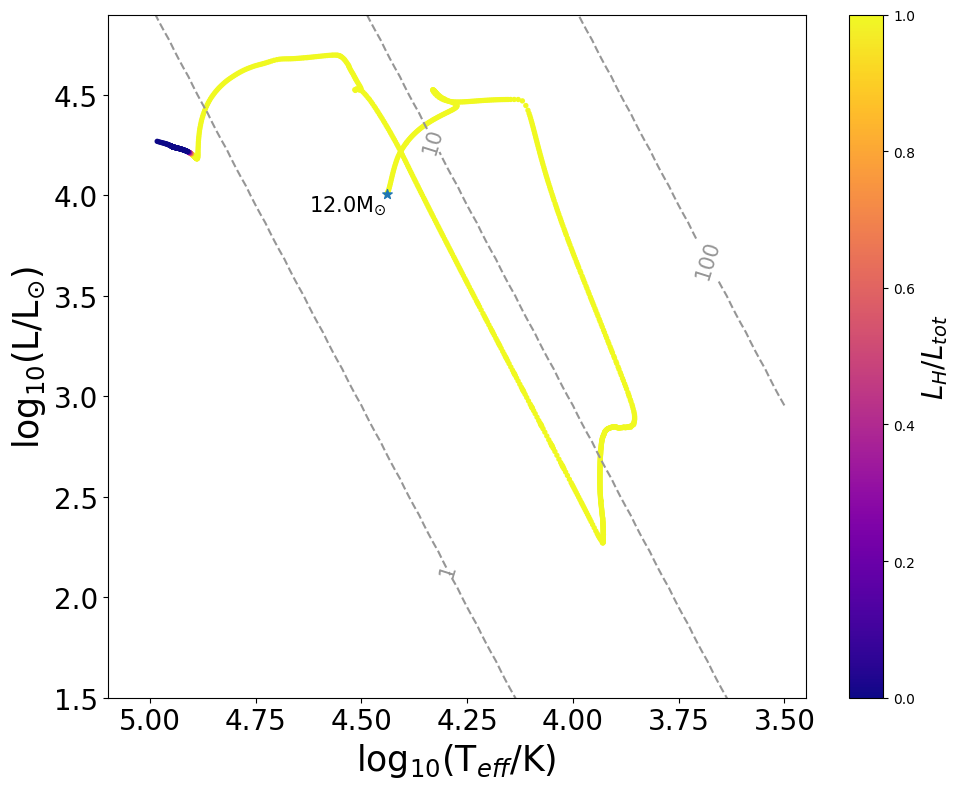
\includegraphics[width=0.45\textwidth]{./plots/HR_log_LH}
\includegraphics[width=0.45\textwidth]{./plots/HR_log_LHe}
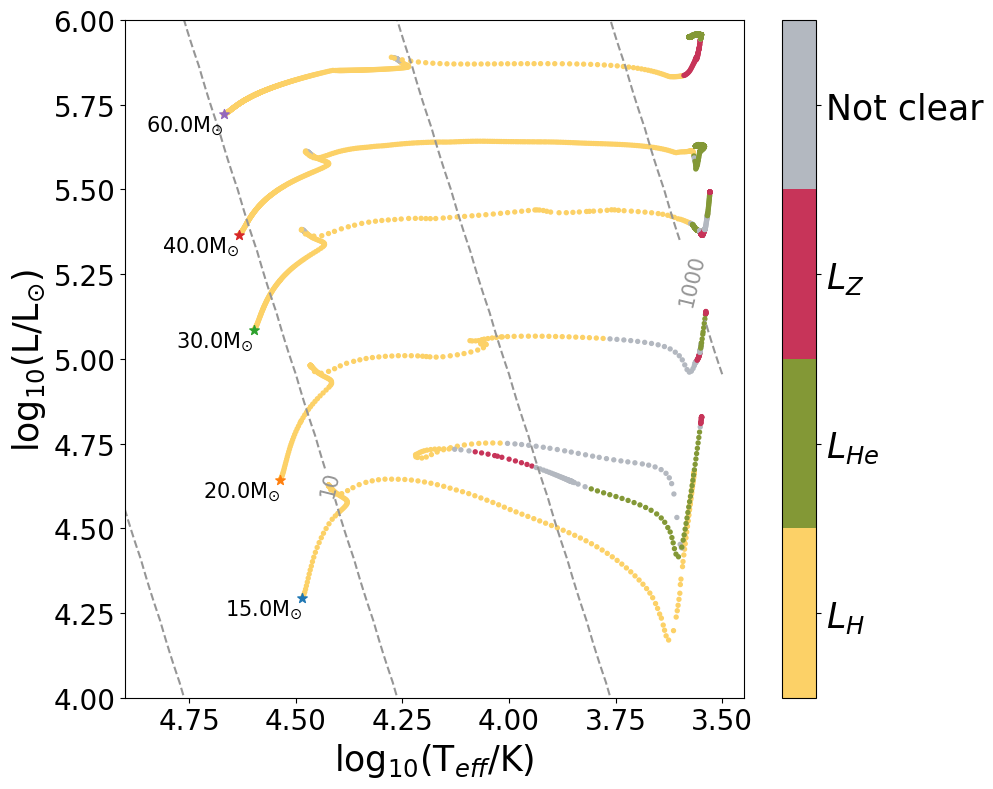
\includegraphics[width=0.45\textwidth]{./plots/HR_log_LZ}
\caption{Problem 1 HRDs of 15, 20, 30, 40, and 60 $\msol$. colored by the fraction of their luminosity  that comes from \textbf{top left:} hydrogen fusion, \textbf{top right:} helium fusion, \textbf{botom:} the  fusion of metals.}
 \label{fig:p1_a}
\end{figure}


In Fig. \ref{fig:p1_a}, we see that hydrogen fusion luminosity dominates during the main sequence (MS), as expected. After stars move along to their post MS phases, helium fusion begins to contribute on a similar level, along with energy production via the fusion of metals. 
If you look carefully, you might have noticed that metal burning appears to contribute to the luminosity earlier than expected (light blue in the bottom plot of  Fig. \ref{fig:p1_a}). This happens during the transitional phase, when the star is moving from H-shel burning to core He burning. At this point, the core He burning is ramping up. This includes Carbon alpha capture ($^{12}C(\alpha, \gamma) ^{16}O$), which MESA counts as a metal burning reaction (while it really shouldn't).
 

\begin{figure}
\center
\includegraphics[width=0.45\textwidth]{./plots/HR_L_dominant}
\caption{Problem 1 HRDs of 15, 20, 30, 40, and 60 $\msol$. coloured by by their dominant luminosity source.  I.e., hydrogen
      fusion (green),  helium fusion (orange), or the fusion of metals (pink). If none of the luminosities dominated more than 50\% of the total luminosity, we label the luminosity as "not clear" (purple).}
    \label{fig:p1_a2}
\end{figure}

Another way to examine this is shown below in Fig. \ref{fig:p1_a2}, where points are coloured according to the dominant source of energy production.
From Fig. \ref{fig:p1_a2} it is immediately apparent that metal and helium fusion only really become dominant sources briefly near the end of the evolution. 
This shows that hydrogen (shell) burning  is the dominant source of the stars luminosity through most of its evolution. There is no clearly dominant source (defined here as one Luminosity contributes more than 50\% of the total luminosity) for significant stretches of the evolution.


%%%%%%%%%%%%%%%%%%%%%%%%%%%%%%%%%%%%%%%%%%%%%%%%%%%%%%%%%%%%%%%%%%%%%%%%%%%%%%%%%%%%%%%%%%%%%%%%%%%%%%%%%%%%%
%%%%%%%%%%%%%%%%%%%%%%%%%%%%%%%%%%%%%% Problem 2 %%%%%%%%%%%%%%%%%%%%%%%%%%%%%%%%%%%%%%%%%%%%%%%%%%%%%%%%%%%%
\vspace{0.1in}
\section{Problem 2}
\vspace{0.1in}

Now we're having a look at the effects of mass loss (according to the so-called ``Dutch'' scheme) on the evolution of our stars from the previous problem. High mass stars may be heavily affected by mass loss, in particular by ``line driven'' mass loss due to their substantial radiation outputs. The more substantial radiation pressure in these stars can carry away layers of the star in a stellar wind, depleting its mass and affecting its evolution.

%%%%%%%%%%%%%%%%%%%%%%%%%%%%%%%%%%% P2: Part (a) %%%%%%%%%%%%%%%%%%%%%%%%%%%%%%%%%%%%%%%%%%%%%%%%%%%%%%%%%%%%
\vspace{0.1in}
\noindent
\textbf{Part (a)}
\vspace{0.1in}

First, let's have a look at how the tracks compare with and without mass loss. Below are HRDs of each of our masses.


\begin{figure}
\center
\includegraphics[width=0.45\textwidth]{./plots/HR_log_abs_mdot15}
\includegraphics[width=0.45\textwidth]{./plots/HR_log_abs_mdot20}
\includegraphics[width=0.45\textwidth]{./plots/HR_log_abs_mdot30}
\includegraphics[width=0.45\textwidth]{./plots/HR_log_abs_mdot40}
\includegraphics[width=0.45\textwidth]{./plots/HR_log_abs_mdot60}
  \caption{Problem 2 (a); HRDs of 15, 20, 30, 40, and 60 $\msol$. Gray dashed lines mark models without mass loss, while coloured lines are coloured by the amount of mass loss that the    model is experiencing.  Mass loss here is according to the Dutch  scheme.}
   \label{fig:p2_a}
\end{figure}

We can see from Fig. \ref{fig:p2_a} that models with mass loss are generally less luminous and cooler than those without mass loss. This is because  removing mass from the star effectively reduces the internal gravity acting on stellar layers, reducing central pressure, therefore temperature, therefore luminosity. In other words, if you strip mass off early enough, the star effectively begins to evolve like a lower mass star because it indeed has less mass. However, we see that above 30 $\msol$ the models that include winds change late evolutionary behaviour and cause the star to 'turn back' towards hotter $T_{eff}$.  Notably, the mass loss in these later stages is substantial, reaching the highest rates of our five models. These stars become Wolf-Rayet stars (as we'll see below), and the temperatures increase substantially in part because much of the H-rich envelope has been
stripped away.


%%%%%%%%%%%%%%%%%%%%%%%%%%%%%%%%%%% P2: Part (b) %%%%%%%%%%%%%%%%%%%%%%%%%%%%%%%%%%%%%%%%%%%%%%%%%%%%%%%%%%%%
\vspace{0.1in}
\noindent
\textbf{Part (b)}
\vspace{0.1in}

Let's continue our analysis by looking at the surface element abundances in our models -- in particular the helium, carbon, and nitrogen abundances. Shown below are the surface abundances for these elements as a function of time.


\begin{figure*}[hbt]
    \plotoneman{plots/p2_b1}{0.4}
    \caption{Problem 2 (b); Helium, carbon, and nitrogen surface
      abundances of 15, 20, 30, 40, and 60 $\msol$ \texttt{MESA}
      stellar models as a function of time to core carbon
      exhaustion. Only the final 80\% of the lifetime is shown, as
      abundance levels remain static prior to this.}
    \label{fig:p2_b1}
\end{figure*}


We can see from Fig. \ref{fig:p2_b1}  the both helium and nitrogen surface abundance rise towards the end of the stars lives, while the abundance of carbon is depleted.  This effect is stronger for increasing mass. This fits with the picture that mass loss is shedding the outer (H-rich) layers of these stars, revealing burning processed material. In particular we see the product of CNO cycling (H burning) which does not only result in He but also enriches the nitrogen abundance and lowers the carbon abundance somewhat (due to the equilibrium speed at which CNO reactions occur). 

The 60$M_{\odot}$ star is an outlier, where the surface abundance of carbon shoots up near the end of the model. This suggests that the winds stripped off enough mass to expose the carbon core. Which matches with our earlier observation that mass loss is heaviest for the  60 $\msol$ case.

Wolf-Rayet (WR) stars are distinguished by having high levels of helium and nitrogen or carbon in their surface composition. It is believed that these stars represent O type stars that have undergone severe mass loss, revealing the inner layers of their structure, like our models here appear to show.  Continuing our analysis, we can look at the HRDs of these models coloured by surface hydrogen, helium abundance, and the ratios of nitrogen to carbon surface abundances. This information is displayed in Fig.  \ref{fig:p2_b2} below.

\begin{figure}
\center
\includegraphics[width=0.45\textwidth]{./plots/HR_surface_he4}
\includegraphics[width=0.45\textwidth]{./plots/HR_N_C}
    \caption{Problem 2 (b); HRDs of 15, 20, 30, 40, and 60 $\msol$  \texttt{MESA} stellar models, coloured by surface helium (left) and nitrogen to carbon ratio (right) surface abundances. The red hatched region shows roughly where Wolf-Rayet stars might be expected, based on the surface H abundance.}
    \label{fig:p2_b2}
\end{figure}


WR stars are often identified by a relatively low surface hydrogen abundance ($X<0.3$, see red hatched region in Figure \ref{fig:p2_b2}), and are sub-divided into two classes: WN (high surface N abundance) and WC (high C abundance). From Fig. \ref{fig:p2_b2},  we expect to see WR stars in a region roughly of log $T_{\rm{eff}} > 4.5$ [K] and log $L > 5.75$ [$L_{\odot}$], or in the hatched region shown in Fig. \ref{fig:p2_b2}. At the end of the 60 $\msol$ track, we see the N/C ratio drop, as the surface C abundance rises dramatically in this phase, as seen in Fig \ref{fig:p2_b1}.

%%%%%%%%%%%%%%%%%%%%%%%%%%%%%%%%%%%%%%%%%%%%%%%%%%%%%%%%%%%%%%%%%%%%%%%%%%%%%%%%%%%%%%%%%%%%%%%%%%%%%%%%%%%%%
%%%%%%%%%%%%%%%%%%%%%%%%%%%%%%%%%%%%%% Problem 3 %%%%%%%%%%%%%%%%%%%%%%%%%%%%%%%%%%%%%%%%%%%%%%%%%%%%%%%%%%%%
\newpage
\vspace{0.1in}
\section{Problem 3}
\vspace{0.1in}

Binary stellar systems are common, especially for high mass stars. Here we're exploring the probability that our models computed in the previous problems might interact with a binary companion over its lifetime. 

Binary interaction is deemed to happen when the primary (higher or equal mass) star's radius expands beyond its Roche lobe radius, $R_L$. At this point, stellar material from the primary star is outside the region where the primary star's gravity dominates, i.e. it is transferring mass to it's companion. 

The question: "what is the probability a star will have interacted with a companion, at each point of the stars' evolution?" is the same as asking: "What is the probability that $R_{\star}$ = $R_{RL}$?". \\

We are given equations for the Roche lobe radius ( $R_{RL}$), orbital period, and the probability distributions of the mass ratio and log orbital period for binary systems. $R_{\star}$ changes over the evolution of the star, and so does its mass, hence our condition fro $R_{RL}$ wil also change.

We are given the Roche lobe radius as approximated by Eggleton 1983:

\begin{equation}
R_{RL,1} = a \frac{0.49 x^{2/3}}{0.6 x^{2/3} + ln(1 + x^{1/3})}
\end{equation}
with $x \equiv q^{-1} \equiv m_2/m_1$.\\

If you choose to use Monte Carlo sampling,  you should draw a number of log orbital periods and mass ratios in the respective intervals [0.15, 3.5] days, and [0.1, 1.0]. The probability of interaction is calculated as the fraction of samples that satisfy the condition $R_1 \geq R_{RL}$. Make sure to sample enough to avoid stochastic noise (of the order of $10^4$ companions should do the trick).\\

However, you can avoid stochastic noise all together by calculating this analytically!

For simplicity, let's go ahead and call 
\begin{equation}
f_{eggle}(q) \equiv \frac{0.49 x^{2/3}}{0.6 x^{2/3} + ln(1 + x^{1/3})}
\end{equation}

Using Kepler we can re-write the  $R_{RL}$ radius to

\begin{equation}
 R_{\star} \leq R_{RL,1} = \left( P^2 \frac{G m_1(1+q)}{(2\pi)^2} \right)^{1/3} f_{eggle}(q) \end{equation}


So given a mass ratio q, we can calculate the required period for $R_{\star}$ to be equal to $R_{RL}$

\begin{equation}
 P_{RL}   = \left[  \frac{(2\pi)^2}{G m_1(1+q)} \left(\frac{R_{RL,1}}{f_{eggle}(q)}\right)^{3} \right]^{1/2}
 \label{eq:PRL}
\end{equation}

Since we now have the period required for RLOF ($P_{RL}$) as a function of the mass ratio, we can calculate the required period over a range of mass ratio's. You should always make sure that you exclude 'non-physical' periods, i.e. $P_{RL}$ outside of our allowed period regime $0.15 < \log P_{RL}< 3.5$.

With this we can estimate the probabillity ($Prob(P,q, f_{bin}$), see below) for each P and q combination. 
We are told that the initial mass ratio distribution is flat:

\begin{equation}
f_{q} = q^0 = 1
\end{equation}
with $0.1<q<1.0$

the initial period distribution 
\begin{equation}
f_{\log_{10} P} = \log_{10} P^{-0.5}
\end{equation}
with $0.15 < \log_{10} P< 3.5$

The fraction of systems with a certain logP or lower is thus
\begin{equation}
Prob(\log_{10} P) = \frac{ \int_{0.15}^{\log_{10}P} (\log_{10} P)^{-0.5} }{\int_{0.15}^{3.5} (\log_{10} P)^{-0.5}}
\end{equation}

\begin{equation}
Prob(\log_{10} P) = \frac{ (\log_{10} P)^{0.5} - 0.15^{0.5} }{ 3.5^{0.5} - 0.15^{0.5} }
\end{equation}

similar but easier for q, but here we need some mass ratio q, or higher for $ R_{\star} \leq R_{RL,1}$ :

\begin{equation}
Prob(q) = \frac{ 1-q }{ 0.9 }
\end{equation}

Finally, the binary fraction is $f_{bin} = 0.7$.
The total probability of a certain configuration is thus:

\begin{equation}
Prob(\log P, q, f_{bin}) = Prob(q) \cdot Prob(\log P) \cdot f_{bin}
\end{equation}

So using all this we will calculate, for each mass ratio, the required period $P_{RL}$ (equation \ref{eq:PRL}) and corresponding probability to form such a system.
Since everything is a function of the mass ratio now, we just have to calculate the probabilities for a range of q, and then take the maximum value. Again, make sure that you exclude 'impossible' values of P from this calculation, i.e. set the probability to zero in that case!.


\begin{figure*}
\center
\includegraphics[width=0.45\textwidth]{./plots/InteractionProb}
\includegraphics[width=0.45\textwidth]{./plots/HR_logprob}
    \caption{Problem 3 (a); Probability of interaction between binary stars for each of our models across their lifetime is shown at       left; HRD with evolutionary tracks of 15, 20, 30, 40, and 60  $\msol$ \texttt{MESA} stellar models, coloured by their log binary interaction probabilities shown at right. }
    \label{fig:p3_a}
\end{figure*}


Generally, the probability of a binary interaction rises for each of our models as time goes on. This makes sense, later on stars inflate after core hydrogen exhaustion, becoming giants. Thus, the probability that an interaction will occur is highest after hydrogen fusion. We also see from Fig. \ref{fig:p3_a} that the probability of interaction is generally larger for larger initial mass. This makes sense too, since higher mass stars tend to be more tenuous and inflated objects, increasing the likelihood of a Roche lobe overflow for a greater range of binary companion masses. 

In summary, for massive stars, the probability of binary interaction is modest on the main sequence but very high in post-main sequence evolutionary phases!

\end{document}
